\chapter{Hintergrund} % (fold)
\label{cha:hintergrund}
Zum allgemeinen Verständnis erklärt dieses Kapitel das grundlegenden Konzept von CBM und dient als Basis für die folgenden Kapitel. Hierbei wird nur auf die für den Algorithmus relevanten Aspekte eingegangen. 

Beim CBM werden Karten als Notationselemente verwendet. Dabei wird zwischen drei Typen unterschieden:
\begin{description}
	\item[Subjekt - BLAU] repräsentiert eine Person/Rolle im Prozess welchem Aufgaben zugeordnet werden.
	\item[Aufgabe - ROT] repräsentiert eine ausführbare Aktion die von Subjekten durchgeführt werden.
	\item[Transfer - GELB] entsprechen Nachrichten zwischen Subjekten/Aufgaben und stellen den Kommunikationsfluss dar.
\end{description}

Abbildung \ref{fig:cbm-grundstruktur} zeigt ein beispielhaftes Modell nach CBM. Für den hier vorgestellten Algorithmus sind die grün umrandeten Elemente von Bedeutung. Jedes der Rechtecke beinhaltet ein Subjekt (blau) als Startelement und sequenziell in chronologischer Reihenfolge angeordnete Aufgaben (rot). Die Abhängigkeiten bzw. Transferelemente (gelb) zwischen den Subjekten sind für den Algorithmus nicht von Bedeutung. Der Algorithmus soll ausschließlich die Zuordnung von Subjekten zu Aufgaben bestimmen.
\begin{figure}[H]
	\centering 
	\begin{minipage}[b]{0.9\textwidth} 
		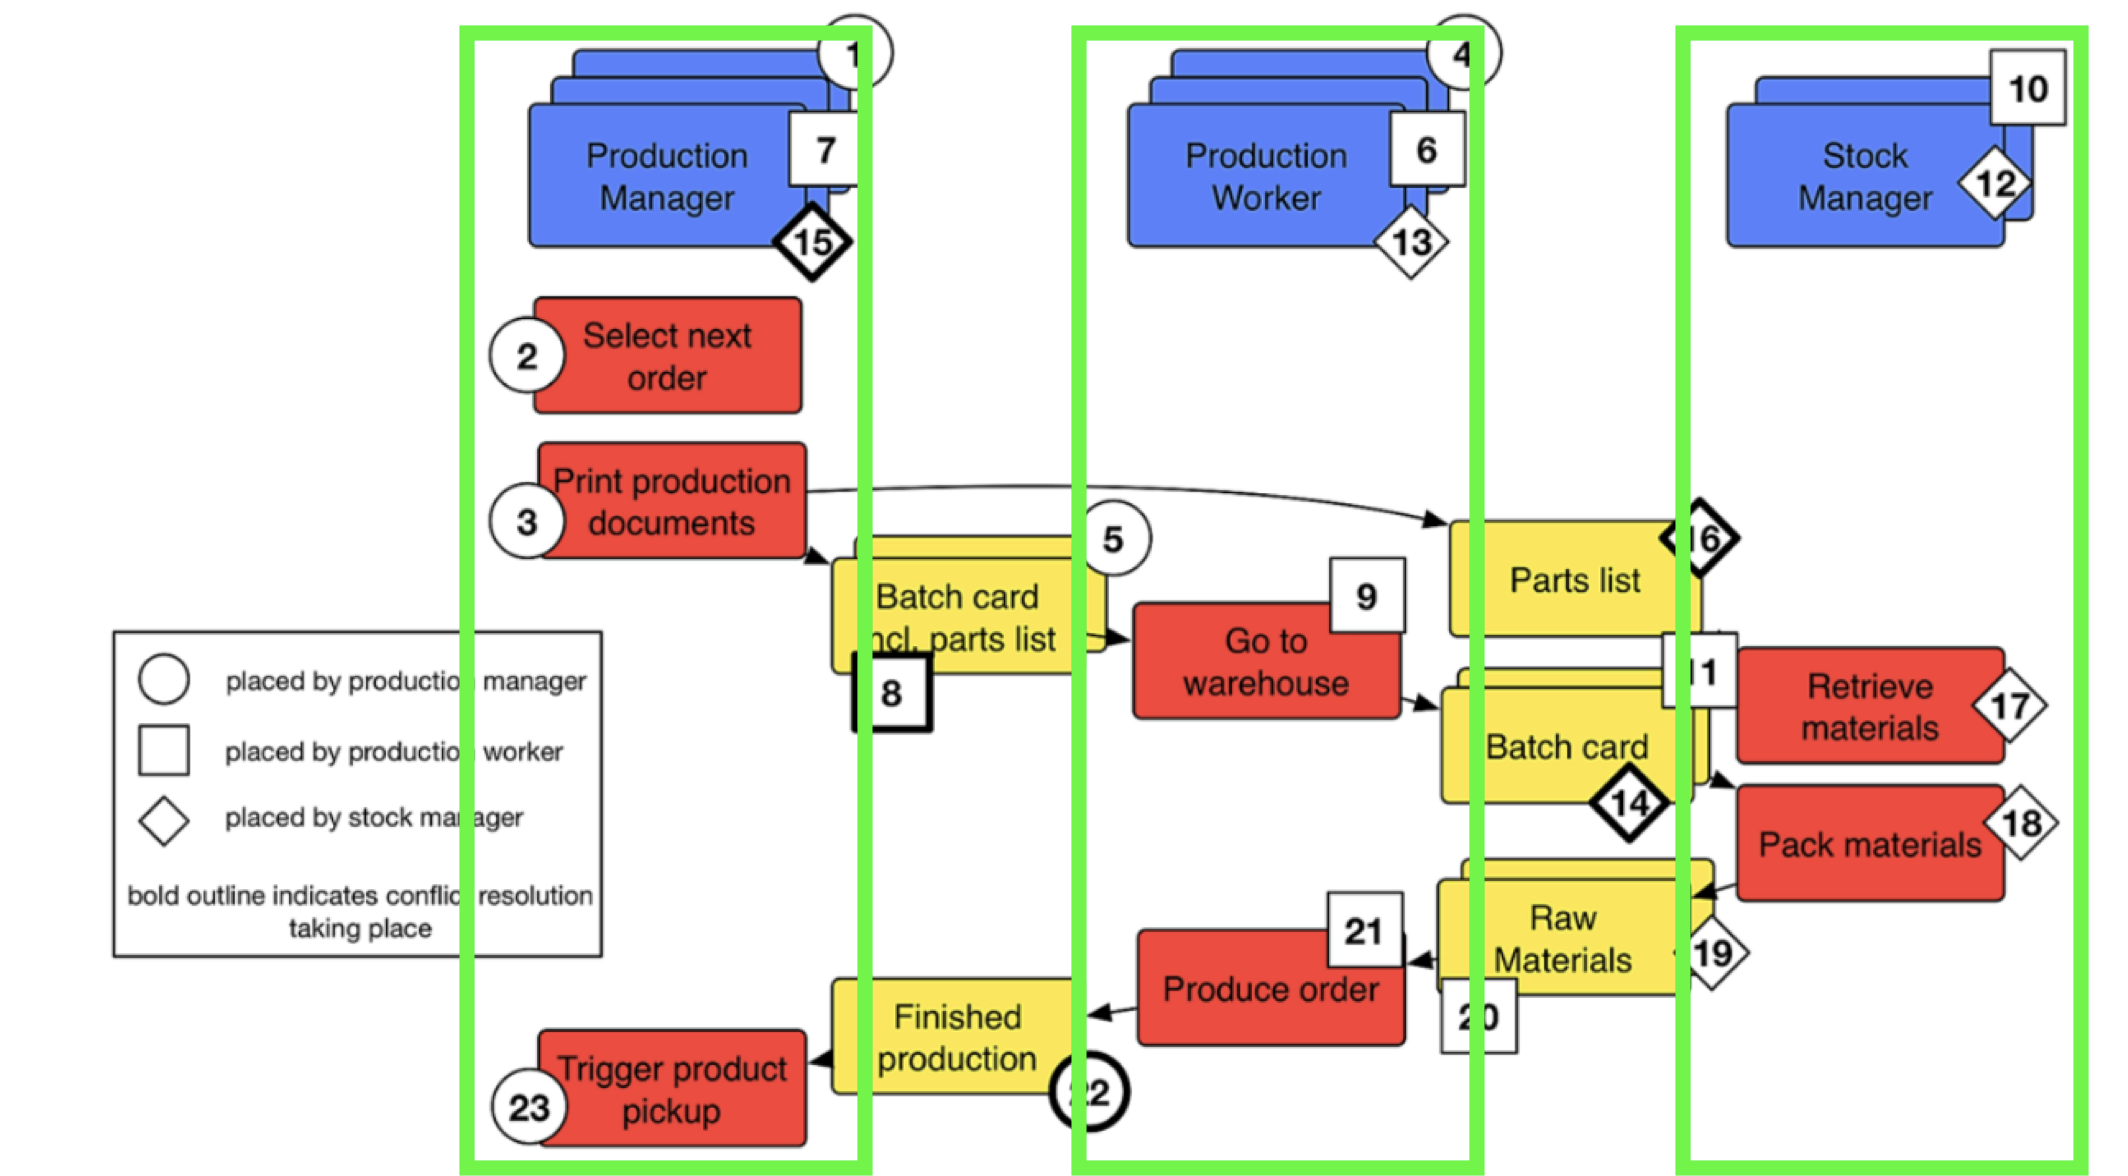
\includegraphics[width=\textwidth]{figures/cbm-grundstruktur.png} 		\caption{CBM Modell 
		\protect~\cite{oppl2016linking}} 
		\label{fig:cbm-grundstruktur} 
	\end{minipage}
\end{figure}[
% chapter hintergrund (end)